%% 
%% Copyright 2007-2024 Elsevier Ltd
%% 
%% This file is part of the 'Elsarticle Bundle'.
%% ---------------------------------------------
%% 
%% It may be distributed under the conditions of the LaTeX Project Public
%% License, either version 1.3 of this license or (at your option) any
%% later version.  The latest version of this license is in
%%    http://www.latex-project.org/lppl.txt
%% and version 1.3 or later is part of all distributions of LaTeX
%% version 1999/12/01 or later.
%% 
%% The list of all files belonging to the 'Elsarticle Bundle' is
%% given in the file `manifest.txt'.
%% 
%% Template article for Elsevier's document class `elsarticle'
%% with harvard style bibliographic references

\documentclass[preprint,12pt,authoryear]{elsarticle}

%% Use the option review to obtain double line spacing
%% \documentclass[authoryear,preprint,review,12pt]{elsarticle}

%% Use the options 1p,twocolumn; 3p; 3p,twocolumn; 5p; or 5p,twocolumn
%% for a journal layout:
%% \documentclass[final,1p,times,authoryear]{elsarticle}
%% \documentclass[final,1p,times,twocolumn,authoryear]{elsarticle}
%% \documentclass[final,3p,times,authoryear]{elsarticle}
%% \documentclass[final,3p,times,twocolumn,authoryear]{elsarticle}
%% \documentclass[final,5p,times,authoryear]{elsarticle}
%% \documentclass[final,5p,times,twocolumn,authoryear]{elsarticle}

%% For including figures, graphicx.sty has been loaded in
%% elsarticle.cls. If you prefer to use the old commands
%% please give \usepackage{epsfig}

%% The amssymb package provides various useful mathematical symbols
\usepackage{amssymb}
%% The amsmath package provides various useful equation environments.
\usepackage{amsmath}
%% The amsthm package provides extended theorem environments
%% \usepackage{amsthm}
\usepackage{url}
\usepackage{graphicx}
%% The lineno packages adds line numbers. Start line numbering with
%% \begin{linenumbers}, end it with \end{linenumbers}. Or switch it on
%% for the whole article with \linenumbers.
%% \usepackage{lineno}

\journal{Climate Services}

\begin{document}

\begin{frontmatter}

%% Title, authors and addresses

%% use the tnoteref command within \title for footnotes;
%% use the tnotetext command for theassociated footnote;
%% use the fnref command within \author or \affiliation for footnotes;
%% use the fntext command for theassociated footnote;
%% use the corref command within \author for corresponding author footnotes;
%% use the cortext command for theassociated footnote;
%% use the ead command for the email address,
%% and the form \ead[url] for the home page:
%% \title{Title\tnoteref{label1}}
%% \tnotetext[label1]{}
%% \author{Name\corref{cor1}\fnref{label2}}
%% \ead{email address}
%% \ead[url]{home page}
%% \fntext[label2]{}
%% \cortext[cor1]{}
%% \affiliation{organization={},
%%            addressline={}, 
%%            city={},
%%            postcode={}, 
%%            state={},
%%            country={}}
%% \fntext[label3]{}

\title{Supplementary Materials for ``Balancing Accuracy versus Precision: Enhancing the Usability of Sub-Seasonal Forecasts"} %% Article title

%% use optional labels to link authors explicitly to addresses:
%% \author[label1,label2]{}
%% \affiliation[label1]{organization={},
%%             addressline={},
%%             city={},
%%             postcode={},
%%             state={},
%%             country={}}
%%
%% \affiliation[label2]{organization={},
%%             addressline={},
%%             city={},
%%             postcode={},
%%             state={},
%%             country={}}


\author[label1,label2]{Etienne Dunn-Sigouin} %% Author name
\ead{etdu@norceresearch.no}


\author[label1,label2]{Erik W. Kolstad}


\author[label1,label2]{C. Ole Wulff}

\author[label1,label2,label3,label4]{Douglas J. Parker}

\author[label3,label5]{Richard J. Keane}


%% Author affiliation
\affiliation[label1]{organization={NORCE Norwegian Research Center AS},%Department and Organization 
            city={Bergen},
            country={Norway}}

\affiliation[label2]{organization={Bjerknes Center for Climate Research},%Department and Organization 
            city={Bergen},
            country={Norway}}

\affiliation[label3]{organization={School of Earth and Environment, University of Leeds},%Department and Organization 
            city={Leeds},
            country={UK}}

\affiliation[label4]{organization={NCAS National Centre for Atmospheric Science, University of Leeds},%Department and Organization 
            city={Leeds},
            country={UK}}

\affiliation[label5]{organization={Met Office},%Department and Organization 
            city={Exeter},
            country={UK}}
            
%% Abstract
%\begin{abstract}
%% Text of abstract


%\end{abstract}

%%Graphical abstract
%\begin{graphicalabstract}
%\includegraphics{grabs}
%\end{graphicalabstract}

%%Research highlights
%\begin{highlights}
%\item blablabla
%\end{highlights}

%% Keywords
%\begin{keyword}
%% keywords here, in the form: keyword \sep keyword
%sub-seasonal forecasts \sep usability gap \sep forecast skill horizon \sep climate adaptation \sep ECMWF \sep fractions skill score
%% PACS codes here, in the form: \PACS code \sep code

%% MSC codes here, in the form: \MSC code \sep code
%% or \MSC[2008] code \sep code (2000 is the default)

%\end{keyword}

\end{frontmatter}

%% Add \usepackage{lineno} before \begin{document} and uncomment 
%% following line to enable line numbers
%% \linenumbers

%% main text
%%

%% Use \section commands to start a section



















%% Refer following link for more details.
%% https://en.wikibooks.org/wiki/LaTeX/Mathematics
%% https://en.wikibooks.org/wiki/LaTeX/Advanced_Mathematics

%% Use a table environment to create tables.
%% Refer following link for more details.
%% https://en.wikibooks.org/wiki/LaTeX/Tables
%\begin{table}[t]%% placement specifier
%% Use tabular environment to tag the tabular data.
%% https://en.wikibooks.org/wiki/LaTeX/Tables#The_tabular_environment
%\centering%% For centre alignment of tabular.
%\begin{tabular}{l c r}%% Table column specifiers
%% Tabular cells are separated by &
 % 1 & 2 & 3 \\ %% A tabular row ends with \\
 % 4 & 5 & 6 \\
 % 7 & 8 & 9 \\
%\end{tabular}
%% Use \caption command for table caption and label.
%\caption{Table Caption}\label{fig1}
%\end{table}



%% Use figure environment to create figures
%% Refer following link for more details.
%% https://en.wikibooks.org/wiki/LaTeX/Floats,_Figures_and_Captions
%\clearpage
%\begin{figure}[t]%% placement specifier
%% Use \includegraphics command to insert graphic files. Place graphics files in 
%% working directory.
%\centering%% For centre alignment of image.
%\includegraphics{example-image-a}
%% Use \caption command for figure caption and label.
%\caption{Figure Caption}\label{fig1}
%% https://en.wikibooks.org/wiki/LaTeX/Importing_Graphics#Importing_external_graphics
%\end{figure}

\newpage
\begin{figure}[t]
  \noindent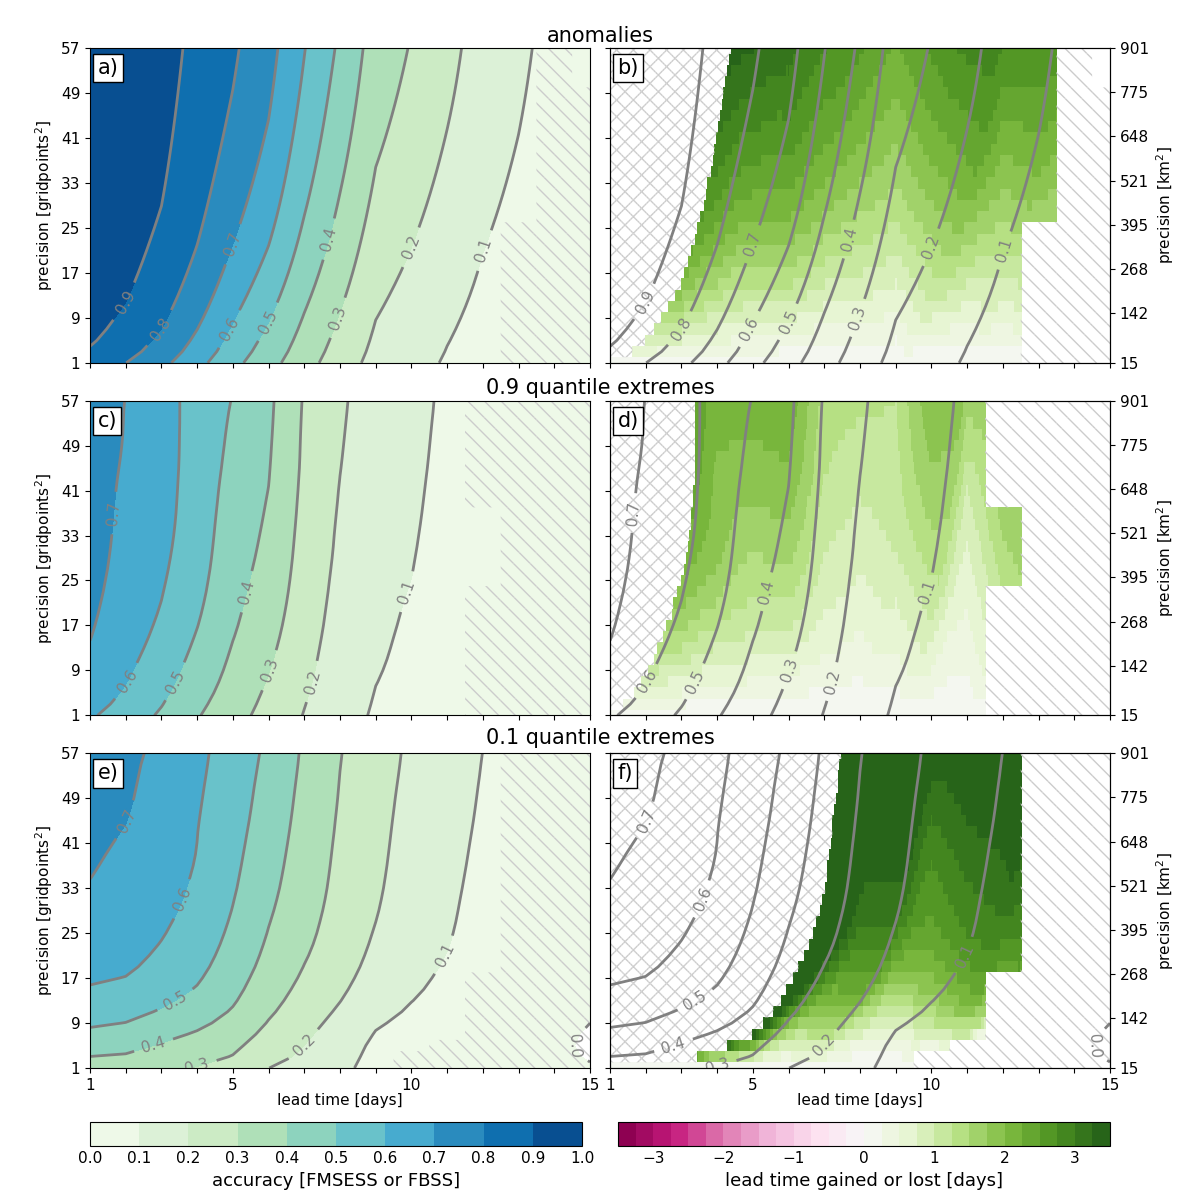
\includegraphics[scale=0.45]{fig_S1.png}\\
  \caption{As in Fig. 1 except for daily-accumulated precipitation forecasts in November-December-January-February-March.}\label{f1}
\end{figure}

\newpage
\begin{figure}[t]
  \noindent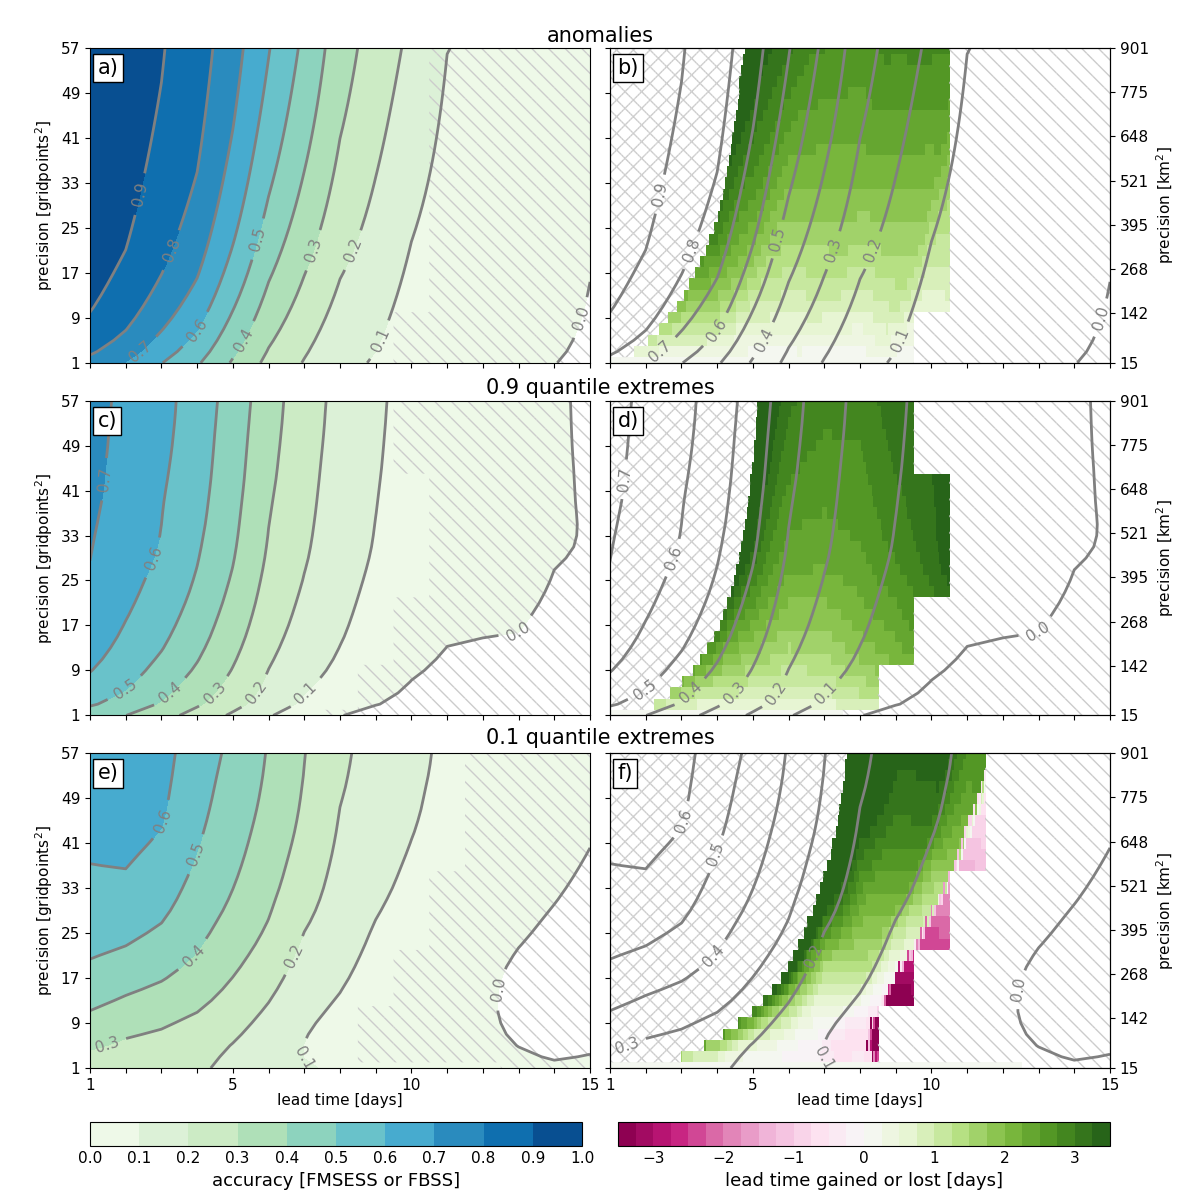
\includegraphics[scale=0.45]{fig_S2.png}\\
  \caption{As in Fig. 1 except for daily-accumulated precipitation forecasts in May-June-July-August-September.}\label{f2}
\end{figure}

\newpage
\begin{figure}[t]
  \noindent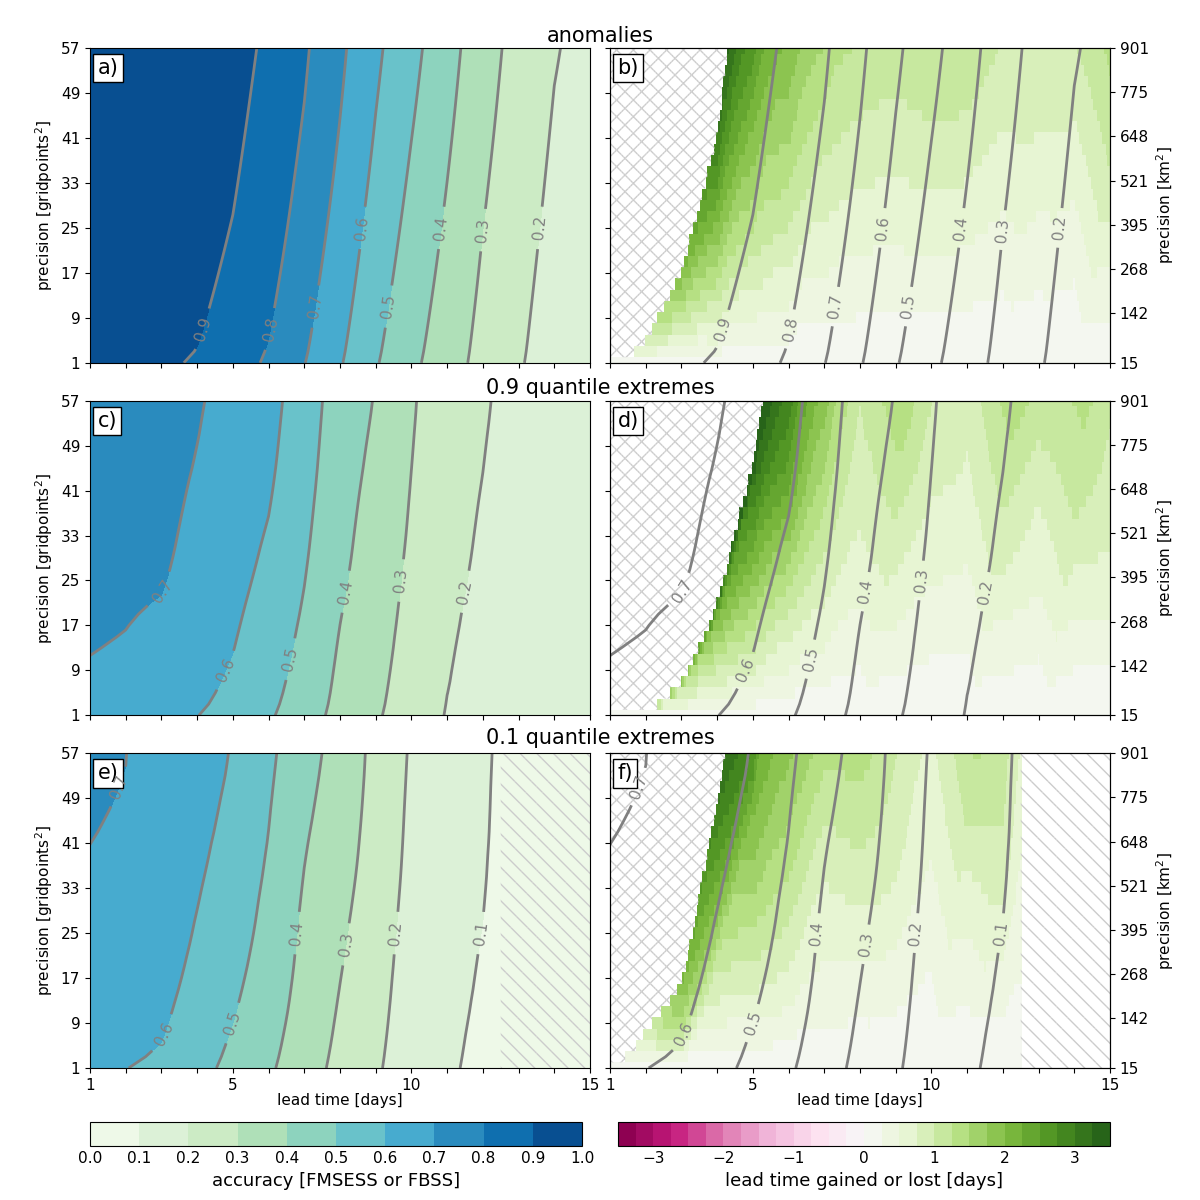
\includegraphics[scale=0.45]{fig_S3.png}\\
  \caption{As in Fig. 1 except for daily-mean 2-meter temperature forecasts.}\label{f3}
\end{figure}

\newpage
\begin{figure}[t]
  \noindent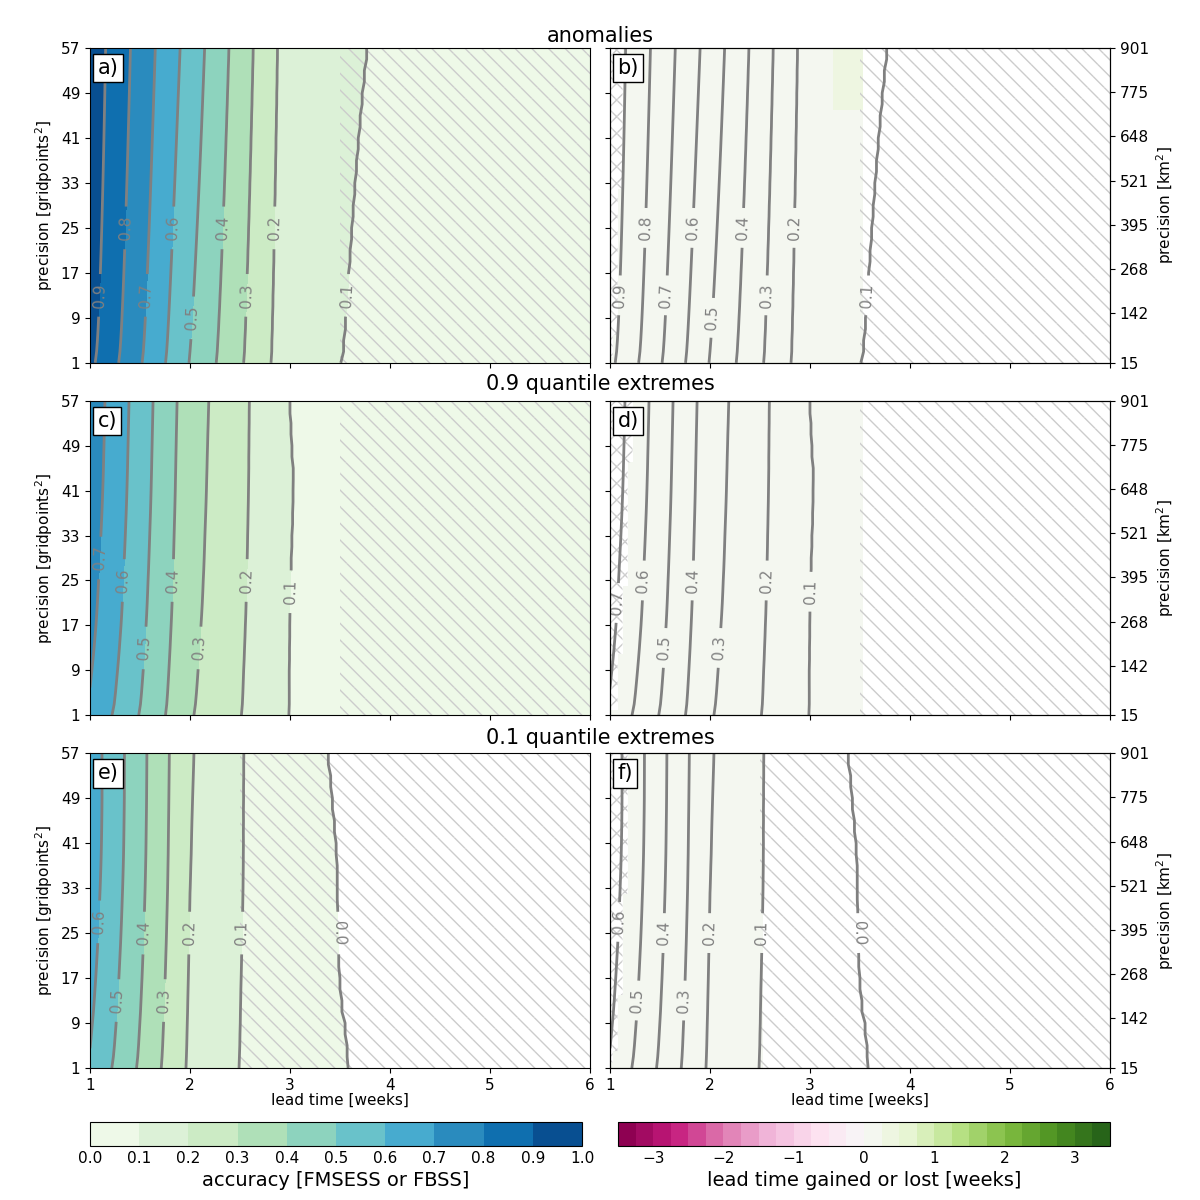
\includegraphics[scale=0.45]{fig_S4.png}\\
  \caption{As in Fig. 3 except for weekly-mean 2-meter temperature forecasts.} \label{f4}
\end{figure}

\newpage
\begin{figure}[t]
  \noindent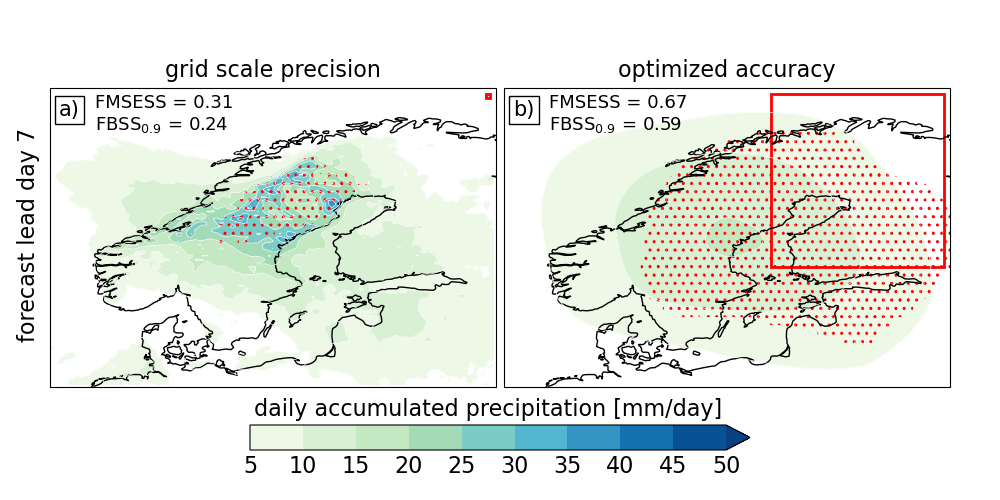
\includegraphics[scale=0.6]{fig_S5.png}\\
  \caption{As in Fig. 6a,b except for forecast lead-day 7.} \label{f5}
\end{figure}


%% The Appendices part is started with the command \appendix;
%% appendix sections are then done as normal sections
%\appendix
%\section{Example Appendix Section}
%\label{app1}

%Appendix text.

%% For citations use: 
%%       \citet{<label>} ==> Lamport (1994)
%%       \citep{<label>} ==> (Lamport, 1994)
%%
%Example citation, See \citet{lamport94}.

%% If you have bib database file and want bibtex to generate the
%% bibitems, please use
%%
%\bibliographystyle{elsarticle-harv} 
%\bibliography{references}

%% else use the following coding to input the bibitems directly in the
%% TeX file.

%% Refer following link for more details about bibliography and citations.
%% https://en.wikibooks.org/wiki/LaTeX/Bibliography_Management

%%\begin{thebibliography}{00}

%% For authoryear reference style
%% \bibitem[Author(year)]{label}
%% Text of bibliographic item

%%\bibitem[Lamport(1994)]{lamport94}
%%  Leslie Lamport,
%%  \textit{\LaTeX: a document preparation system},
%%  Addison Wesley, Massachusetts,
%%  2nd edition,
%%  1994.


%%\end{thebibliography}
\end{document}

\endinput
%%
%% End of file `elsarticle-template-harv.tex'.


